\subsection{Transverter, PTT lines, etc.}
\label{subsec:transverter-ptt}

In this section, we'll explore the world of amplifiers, the driving forces of radio communication that ensure your signal reaches its destination. We'll cover essential components from transceivers to RF power amplifiers, including the important switches that keep everything running smoothly. This will be a brief overview of these topics, providing just enough information to help you pass the exam. We'll explore these topics in greater detail in subsequent books.

\subsubsection*{Transverter: The Frequency Shifter}
A transverter is a nifty device that converts the RF input and output of a transceiver to another band. Think of it as a translator for radio frequencies. If your transceiver operates on one band, but you need to communicate on another, the transverter steps in to make the conversion. It does this by mixing the incoming signal with a local oscillator signal, resulting in a new frequency that matches the desired band. This process is crucial for multi-band operations, allowing you to communicate across different frequency ranges without needing multiple transceivers.

\begin{figure}[h!]
    \centering
    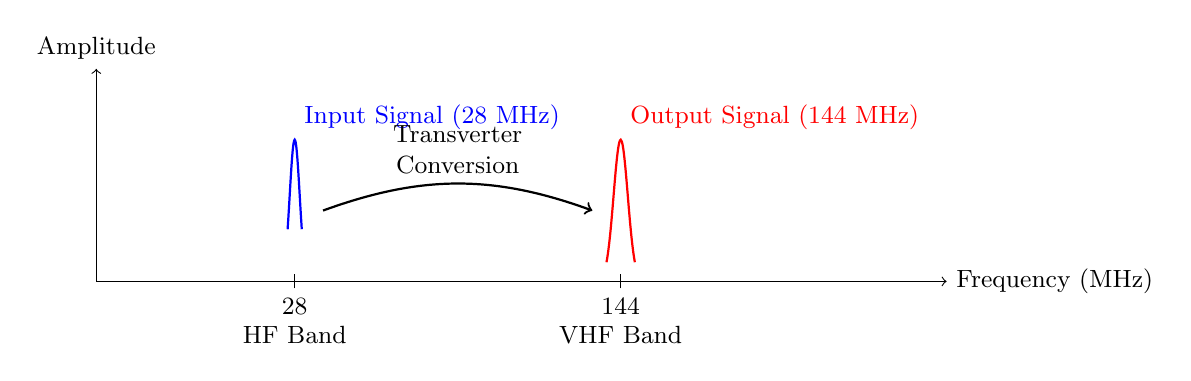
\begin{tikzpicture}[
        scale=0.9,
        every node/.style={font=\small}
    ]
        % Grid settings
        \def\ymax{3}
        \def\xmax{12}
        
        % Axes
        \draw[->] (0,0) -- (\xmax,0) node[right] {Frequency (MHz)};
        \draw[->] (0,0) -- (0,\ymax) node[above] {Amplitude};
        
        % Frequency markers
        \foreach \x/\label in {2.8/28, 7.4/144} {
            \draw (\x,-0.1) -- (\x,0.1);
            \node[below] at (\x,-0.1) {\label};
        }
        
        % Input signal at 28 MHz
        \draw[thick, blue] plot[domain=2.7:2.9,smooth] (\x,{2*exp(-100*(\x-2.8)*(\x-2.8))});
        \node[blue, above right] at (2.8,2) {Input Signal (28 MHz)};
        
        % Output signal at 144 MHz
        \draw[thick, red] plot[domain=7.2:7.6,smooth] (\x,{2*exp(-50*(\x-7.4)*(\x-7.4))});
        \node[red, above right] at (7.4,2) {Output Signal (144 MHz)};
        
        % Conversion arrow
        \draw[->, thick] (3.2,1) to[bend left=20] 
            node[midway, above, text width=2cm, align=center] {Transverter\\Conversion} (7,1);
            
        % Optional: Add frequency bands labels
        \node[below] at (2.8,-0.5) {HF Band};
        \node[below] at (7.4,-0.5) {VHF Band};
        
    \end{tikzpicture}
    \caption{Frequency spectrum showing signal conversion by a transverter from 28 MHz (HF) to 144 MHz (VHF) band}
    \label{fig:transverter-signals}
\end{figure}

\subsubsection*{PTT (Push-to-Talk): The Transmit/Receive Switch}
Next up is the PTT input, a critical feature in transceivers. The PTT input is what switches your transceiver from receive mode to transmit mode when grounded. In simpler terms, when you press the PTT button (usually on your microphone), it grounds the PTT input, telling the transceiver, "Hey, it's time to transmit!" When you release the button, the transceiver goes back to listening mode. This mechanism ensures that you're not transmitting and receiving at the same time, which would be... well, chaotic.


\subsubsection*{Modulation: The Voice of Radio}
Modulation is how we combine our voice or data with a radio signal for transmission. Think of it like writing a message, where we have three different ways to vary our writing:

\begin{itemize}[noitemsep]
    \item \textbf{Amplitude Modulation (AM):} Like changing how hard you press the pencil while writing. The height (strength) of the radio wave changes based on your voice - louder voice makes taller waves, softer voice makes shorter waves.
    
    \item \textbf{Frequency Modulation (FM):} Like changing how quickly you write each letter. The radio wave bunches up or spreads out based on your voice - louder parts make the waves bunch closer together, softer parts spread them apart.
    
    \item \textbf{Phase Modulation (PM):} Like slightly shifting each letter forward or backward while writing. The timing of each radio wave peak shifts slightly based on your voice - similar to FM but responds to how quickly your voice changes rather than its volume.
\end{itemize}

Each method has its advantages: AM is simple but picks up noise easily, FM gives better quality and is less affected by noise (which is why it's used for music radio), and PM is particularly useful for digital signals.

\begin{figure}[h!]
    \centering
    \includegraphics[width=0.9\textwidth]{images/modulations.png}
    \caption{Comparison of different modulation types: Amplitude Modulation (AM) varies the signal amplitude,  Frequency Modulation (FM) varies the signal frequency, and  Phase Modulation (PM) varies the signal phase according to the modulating signal}
    \label{fig:modulation-comparison}
\end{figure}


\subsubsection{Questions}
\begin{tcolorbox}[colback=gray!10!white,colframe=black!75!black,title={T7A06}]
    What device converts the RF input and output of a transceiver to another band?
    \begin{enumerate}[label=\Alph*),noitemsep]
        \item High-pass filter
        \item Low-pass filter
        \item \textbf{Transverter}
        \item Phase converter
    \end{enumerate}
\end{tcolorbox}
A transverter is specifically designed to convert RF signals from one band to another, making it the correct answer. High-pass and low-pass filters are used to filter frequencies, not convert them, and a phase converter is unrelated to frequency conversion.

\begin{tcolorbox}[colback=gray!10!white,colframe=black!75!black,title={T7A07}]
    What is the function of a transceiver’s PTT input?
    \begin{enumerate}[label=\Alph*),noitemsep]
        \item Input for a key used to send CW
        \item \textbf{Switches transceiver from receive to transmit when grounded}
        \item Provides a transmit tuning tone when grounded
        \item Input for a preamplifier tuning tone
    \end{enumerate}
\end{tcolorbox}
The PTT input is used to switch the transceiver from receive to transmit mode when grounded. It’s not related to CW keys, tuning tones, or preamplifiers.

\begin{tcolorbox}[colback=gray!10!white,colframe=black!75!black,title={T7A08}]
    Which of the following describes combining speech with an RF carrier signal?
    \begin{enumerate}[label=\Alph*),noitemsep]
        \item Impedance matching
        \item Oscillation
        \item \textbf{Modulation}
        \item Low-pass filtering
    \end{enumerate}
\end{tcolorbox}
Modulation is the process of combining speech with an RF carrier signal. Impedance matching, oscillation, and low-pass filtering are unrelated to this process.
